\documentclass[../main.tex]{subfiles}

\begin{document}

\chapter{Introduction}
Optical flats are precision devices used in the field of material science to measure the flatness of surfaces or to create precisely flat surfaces. An optical flat is typically a high-quality, polished, flat glass or quartz disc used in conjunction with monochromatic light to form interference fringes that can be observed and measured to assess surface flatness or quality.\footnote{Optical flats should be handled with great precaution as they are very fragile.} \cite{edmund_optics_optical_flats, kemet_optical_flats, lapmaster_wolters_optical_flats,Paschottaoptical_flats}

\begin{frame}{}
    \begin{figure}[h]
        \centering
        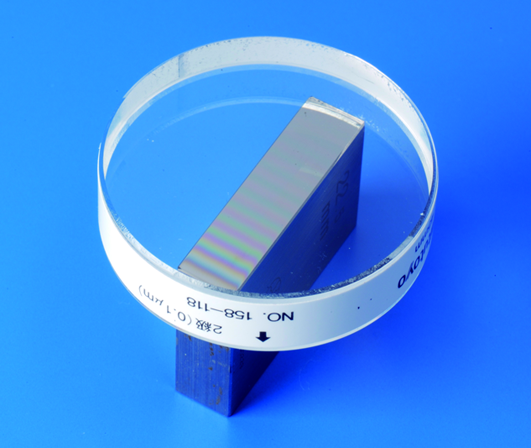
\includegraphics[width=0.8\textwidth]{Images/Introduction/optical_flat}
        \caption{Example of an optical flat \cite{optical_flat_mitutoyo}}
        \label{fig:optical_flat_example}
    \end{figure}
\end{frame}

\section{Physical Characteristics}
\subsection{Material Composition}
Optical flats are predominantly made from two types of materials: fused silica and ultra-low expansion (ULE) glass. Fused silica, known for its exceptional optical clarity and thermal stability, is ideal for precision measurement tools. It has a very low coefficient of thermal expansion, which means it remains stable under varying temperatures, thereby minimizing measurement errors due to thermal variations.\cite{Paschottafused_silica}

\begin{frame}{}
    \begin{figure}[h]
        \centering
        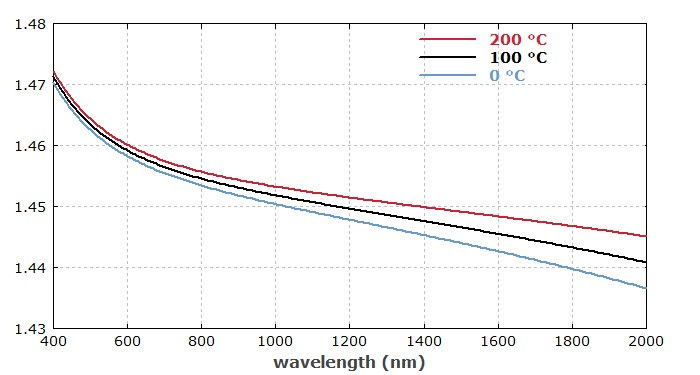
\includegraphics[width=0.8\textwidth]{Images/Introduction/silica_refractive_index}
        \caption{The refractive index of fused silica versus wavelength at three different temperatures.\cite{Paschottafused_silica}}
        \label{fig:refractive_index_silica}
    \end{figure}
\end{frame}

Ultra-low expansion glass, such as Corning's ULE glass, is another favored material. This glass type is engineered to have extremely low thermal expansion rates, which are crucial in maintaining the accuracy of measurements in environments with fluctuating temperatures. ULE glass's robustness and resistance to thermal stress make it particularly suitable for high-precision optical applications, including astronomy and semiconductor manufacturing.\cite{Corning_2022}

Both materials are chosen not only for their minimal thermal properties but also for their ability to be polished to high optical qualities, ensuring that the optical flat does not introduce aberrations or distortions in the interference patterns used for surface measurements.\cite{Corning_2022,Paschottafused_silica,doi:https://doi.org/10.1002/9780470135976.ch1}

\subsection{Surface Quality}
The surface of an optical flat is meticulously polished to achieve a high degree of flatness, typically within fractions of a wavelength of light (\(\lambda/20\) or better). This extreme flatness is crucial for the accuracy of optical measurements. Any imperfections on the surface can distort the interference fringes, leading directly to measurement errors.\cite{enwiki:1212101911}

After the initial polishing phases, optical flats may undergo additional processing steps such as the application of dielectric coatings. These enhancements are critical when the optical flats are used as reference mirrors in precision instruments like the Twyman–Green interferometer, where the utmost flatness is crucial.\cite{Paschottaoptical_flats}

The final quality of optical flats is often verified in an interferometric setup, where they are compared against a reference surface that is of even higher precision. Occasionally, these reference surfaces may utilize fluids like mercury to achieve near-perfect flatness levels, although such materials are challenging to handle and maintain.\cite{Paschottaoptical_flats}

\section{Working Principle}
The principle behind optical flats relies on the optical phenomenon of interference. This section delves into how interference fringes are formed, their types, and their importance in measuring surface characteristics.

\subsection{Interference Fringes}
Interference fringes are the result of the wave nature of light. When monochromatic light—light of a single wavelength—is used to illuminate the interface between an optical flat and another surface, variations in the gap created by surface irregularities cause the waves of light to overlap and interfere with each other. This interference can constructively or destructively affect the light waves, resulting in a pattern of dark and light bands known as interference fringes, which can be observed and analyzed.

\subsubsection{Formation of Fringes}
\begin{frame}{}
    \begin{figure}[H]
        \centering
        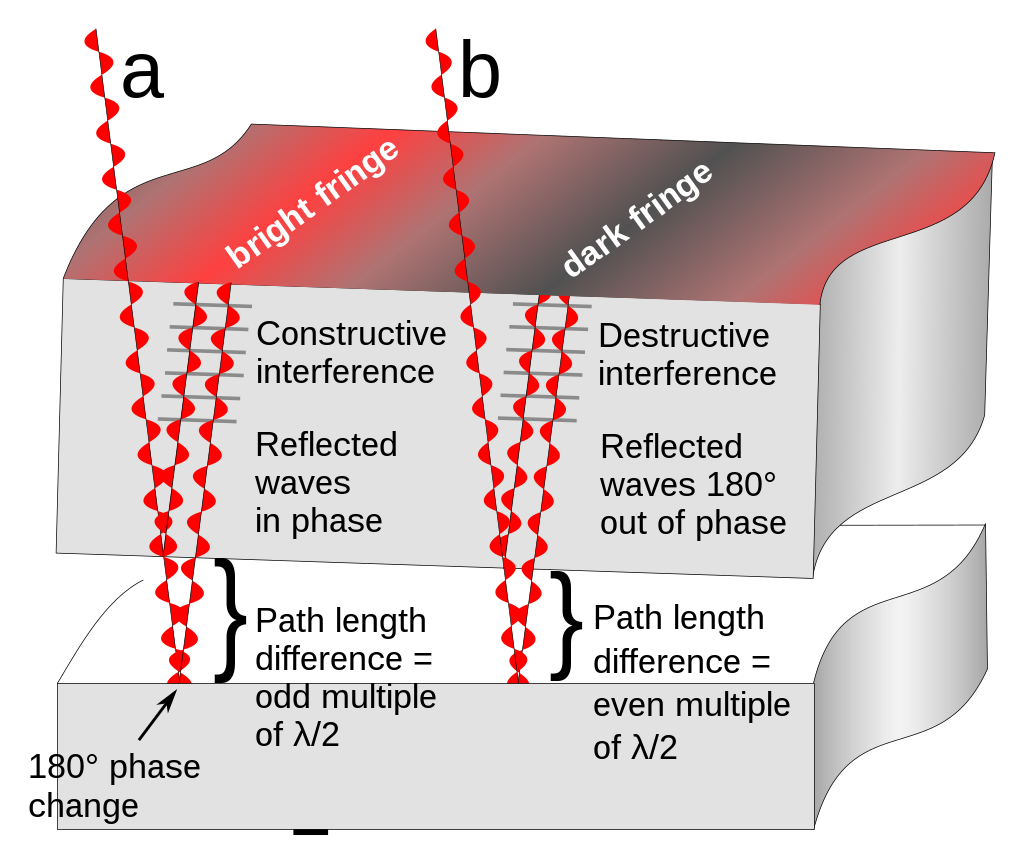
\includegraphics[width=0.8\textwidth]{Images/Introduction/Optical_flat_interference}
        \caption{Formation of interference fringes due to the superposition of light waves.\cite{enwiki:1212101911}}
        \label{fig:interference_fringes}
    \end{figure}
\end{frame}
Consider a setup where an optical flat is placed upon a surface to be tested under a monochromatic light source (figure \ref{fig:interference_fringes}). The light waves reflect off both the bottom surface of the optical flat and the top surface of the test object. Due to differences in the path traveled by the light waves—owing to variations in the gap between the two surfaces—these waves will interfere when they recombine. The condition for constructive and destructive interference is given by the equations:

\begin{equation}
2d \cos(\theta) = m\lambda, \quad \text{(constructive interference)}
\end{equation}
\begin{equation}
2d \cos(\theta) = (m + \frac{1}{2})\lambda, \quad \text{(destructive interference)}
\end{equation}

where:
\begin{itemize}
    \item \(d\) is the gap distance between the optical flat and the test surface,
    \item \(\theta\) is the angle of incidence of the light,
    \item \(m\) is an integer representing the order of the fringe,
    \item \(\lambda\) is the wavelength of the light used.
\end{itemize}

When we dive in deeper on the waves we can see the following: constructive interference occurs when the path difference between the two waves is an integer multiple of the wavelength. Superposition of the waves result in bright fringes.\cite{enwiki:1212101911}

\begin{frame}{}
\begin{figure}[H]
    \centering
    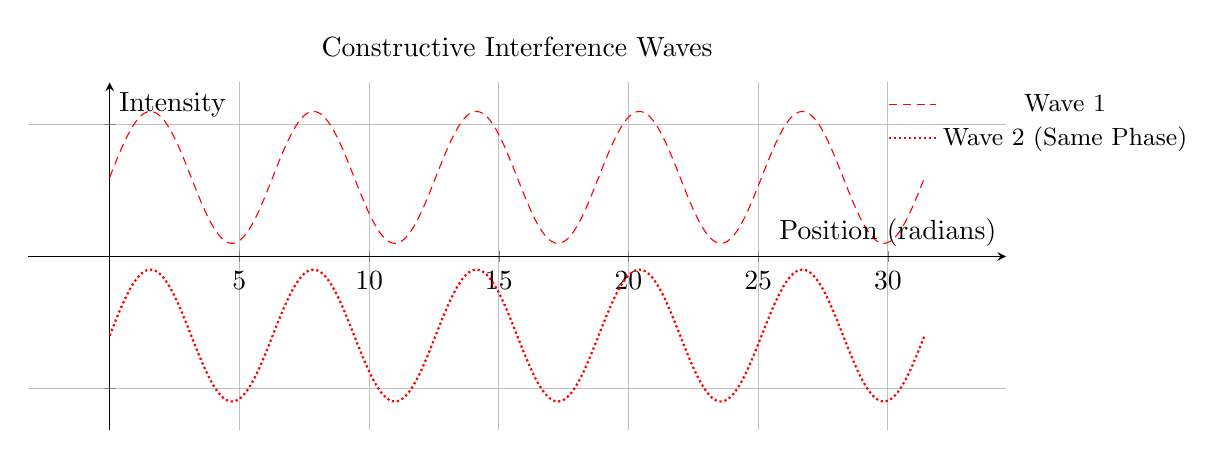
\begin{tikzpicture}
    \begin{axis}[
        title={Constructive Interference Waves},
        xlabel={Position (radians)},
        ylabel={Intensity},
        x label style={at={(axis description cs:1.05,-0.1)},anchor=north},
        yticklabel style={
            /pgf/number format/assume math mode, % This treats labels as math mode
            /pgf/number format/fixed zerofill,    % Adds zeros if needed for padding
            /pgf/number format/precision=1        % Precision of 1 for decimal places
        },
        ytick={},
        yticklabels={}, % Manually specify labels, leaving out -1 and 1
        domain=0:10*pi,
        samples=1000,
        axis lines=middle,
        enlargelimits,
        legend style={
            at={(1.2,1)}, 
            anchor=north east, 
            draw=none, 
            fill=none, 
            text opacity=1, 
            font=\small
        },
        height=6cm, width=14cm,
        grid=major
    ]
        % Wave 1
        \addplot[red, densely dashed] {0.5*sin(deg(x)) + 0.6};
        \addlegendentry{Wave 1}
        % Wave 2
        \addplot[red, densely dotted, thick] {0.5*sin(deg(x)) - 0.6};
        \addlegendentry{Wave 2 (Same Phase)}
        % Resultant Wave
        %\addplot[black] {0.5*sin(deg(x)) + 0.5*sin(deg(x))};
    \end{axis}
    \end{tikzpicture}
    
    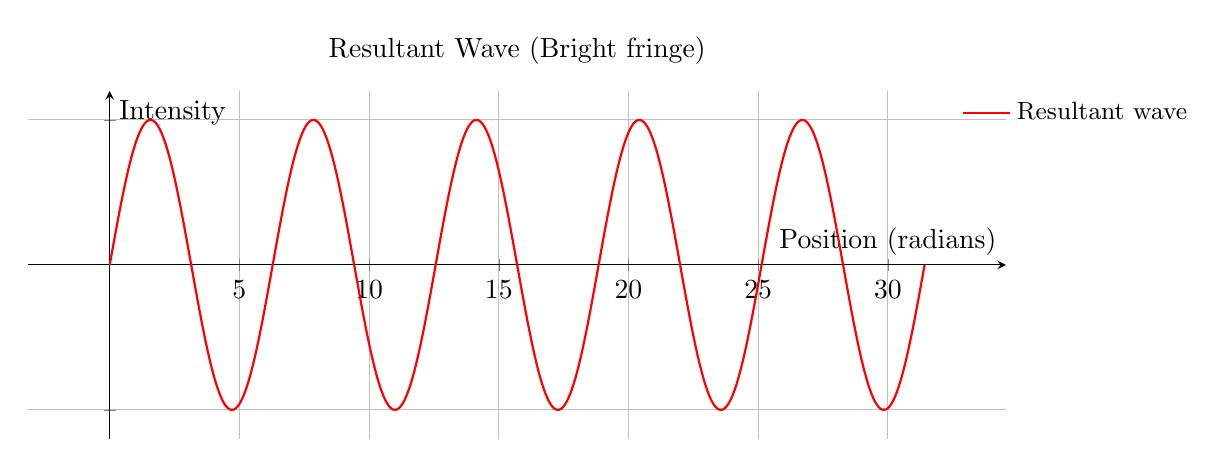
\begin{tikzpicture}
    \begin{axis}[
        title={Resultant Wave (Bright fringe)},
        xlabel={Position (radians)},
        ylabel={Intensity},
        x label style={at={(axis description cs:1.05,-0.1)},anchor=north},
        yticklabel style={
            /pgf/number format/assume math mode,
            /pgf/number format/fixed zerofill,
            /pgf/number format/precision=1
        },
        ytick={},
        yticklabels={},
        domain=0:10*pi,
        samples=1000,
        axis lines=middle,
        enlargelimits,
        height=6cm, width=14cm,
        grid=major,
        legend style={
            at={(1.2,1)}, 
            anchor=north east, 
            draw=none, 
            fill=none, 
            text opacity=1, 
            font=\small
        }
    ]
        % Resultant Wave
        \addplot[red, thick] {0.5*sin(deg(x)) + 0.5*sin(deg(x))};
        \addlegendentry{Resultant wave}
    \end{axis}
    \end{tikzpicture}
    \end{figure}
\end{frame}

Destructive interference, on the other hand, occurs when the path difference is a half-integer multiple of the wavelength, resulting in dark fringes.\cite{enwiki:1212101911}

\begin{frame}{}
    \begin{figure}[H]
        \centering
        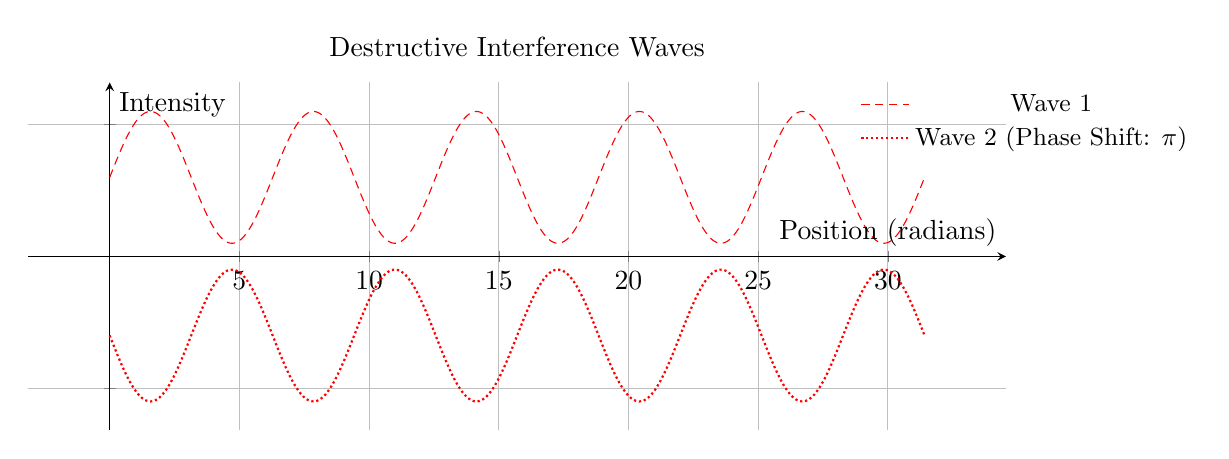
\begin{tikzpicture}
        \begin{axis}[
            title={Destructive Interference Waves},
            xlabel={Position (radians)},
            ylabel={Intensity},
            x label style={at={(axis description cs:1.05,-0.1)},anchor=north},
            yticklabel style={
                /pgf/number format/assume math mode,
                /pgf/number format/fixed zerofill,
                /pgf/number format/precision=1
            },
            ytick={},
            yticklabels={},
            domain=0:10*pi,
            samples=1000,
            axis lines=middle,
            enlargelimits,
            legend style={
                at={(1.2,1)}, 
                anchor=north east, 
                draw=none, 
                fill=none, 
                text opacity=1, 
                font=\small
            },
            height=6cm, width=14cm,
            grid=major
        ]
            % Wave 1
            \addplot[red, densely dashed] {0.5*sin(deg(x)) + 0.6};
            \addlegendentry{Wave 1}
            % Wave 3
            \addplot[red, densely dotted, thick] {0.5*sin(deg(x) + 180) - 0.6};
            \addlegendentry{Wave 2 (Phase Shift: $\pi$)}
        \end{axis}
        \end{tikzpicture}
        
        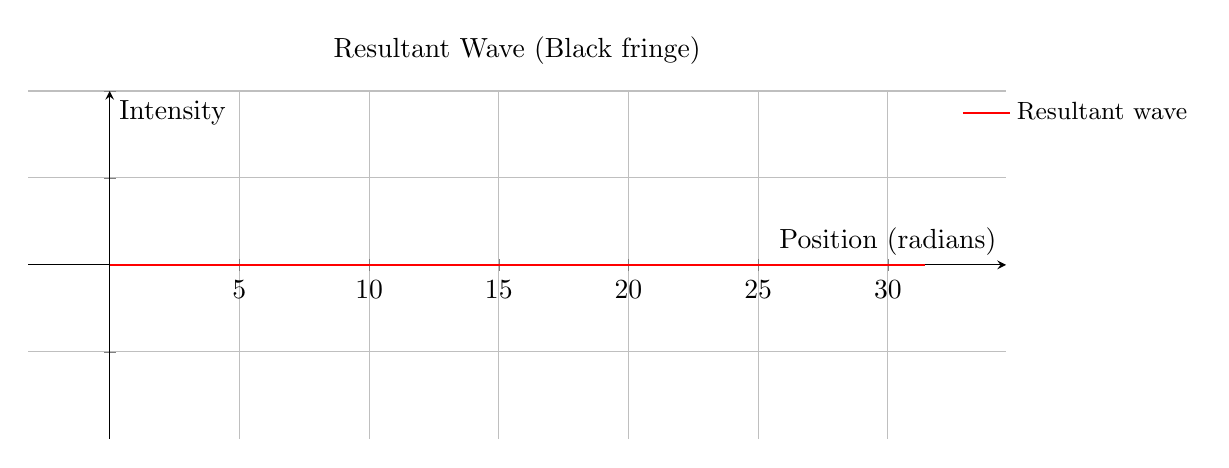
\begin{tikzpicture}
        \begin{axis}[
            title={Resultant Wave (Black fringe)},
            xlabel={Position (radians)},
            ylabel={Intensity},
            x label style={at={(axis description cs:1.05,-0.1)},anchor=north},
            yticklabel style={
                /pgf/number format/assume math mode,
                /pgf/number format/fixed zerofill,
                /pgf/number format/precision=1
            },
            ytick={},
            yticklabels={},
            domain=0:10*pi,
            samples=1000,
            axis lines=middle,
            enlargelimits,
            height=6cm, width=14cm,
            grid=major,
            legend style={
                at={(1.2,1)}, 
                anchor=north east, 
                draw=none, 
                fill=none, 
                text opacity=1, 
                font=\small
            }
        ]
            % Resultant Wave (Destructive)
            \addplot[red, thick] {round(0.5*sin(deg(x)) + 0.5*sin(deg(x) + 180))};
            \addlegendentry{Resultant wave}
        \end{axis}
        \end{tikzpicture}
        \end{figure}
\end{frame}


\subsubsection{Analysis of Fringe Patterns}
The pattern of the fringes provides information about the surface's properties:
\begin{itemize}
    \item \textbf{Straight Fringes} indicate that the test surface is precisely flat. In this scenario, the fringes are parallel and uniformly spaced.
    \item \textbf{Curved Fringes} suggest that the surface is convex or concave. The curvature of the fringes gives clues about the curvature of the surface itself.
    \item \textbf{Irregular Fringes} are indicative of surface defects, bumps, or dips. The irregularity in spacing or the fringe shape can be analyzed to quantify the nature of the surface flaws.
\end{itemize}

\begin{frame}{}
    \begin{figure}[H]
    \centering
    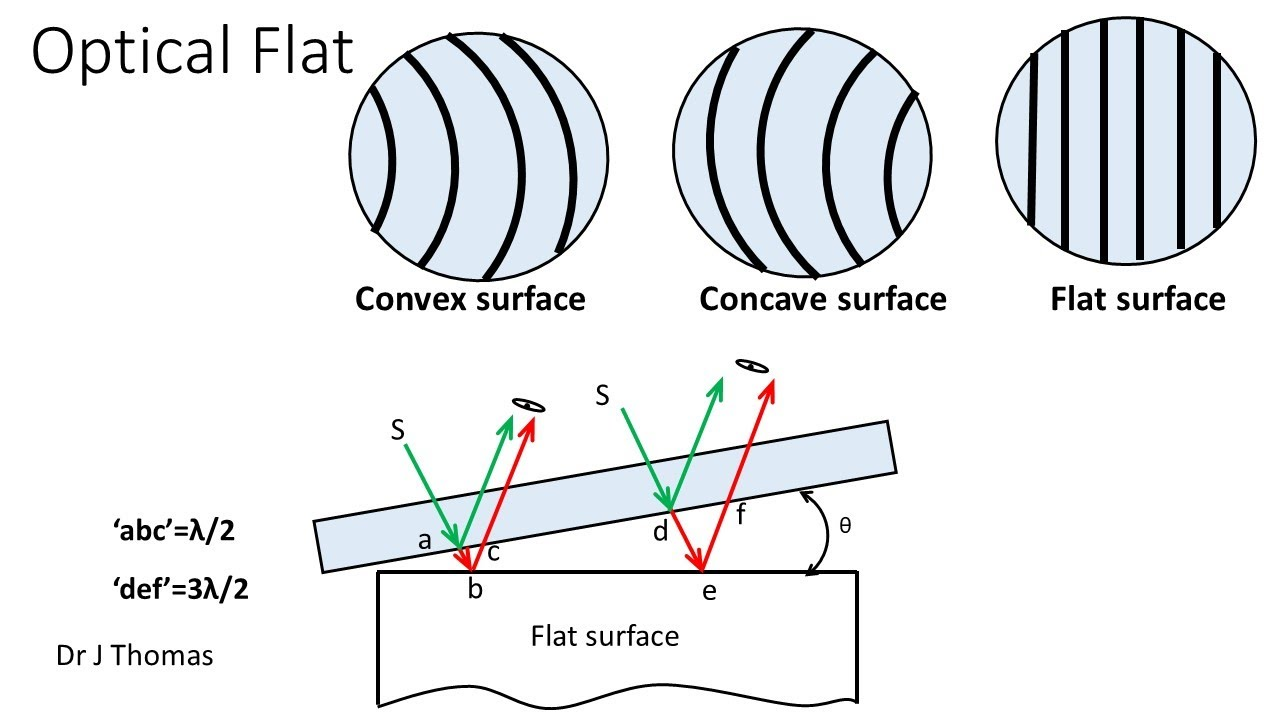
\includegraphics[width=0.8\textwidth]{Images/Introduction/fringe_types}
    \caption{Different types of interference fringe patterns and what they indicate about surface characteristics.\cite{Joji_2023}}
    \label{fig:fringe-types}
    \end{figure}
\end{frame}

\section{Innovations in Optical Flat Technology}
Recent advancements have expanded the traditional concept of optical flats to include plasmonic optical flats, which utilize nanostructured plasmonic surfaces. This innovation stems from the field of plasmonics, where the manipulation of light at the nanoscale allows for extreme localization and sensitivity to environmental changes. Plasmonic optical flats, comprised of nanostructured metal arrays, significantly enhance the sensitivity and resolution of surface inspections beyond the diffraction limit of light. These new optical flats are particularly effective in detecting sub-wavelength surface anomalies and offer the potential for rapid and precise surface inspection using simple, low-cost equipment.

\subsection{Advancements in Metrology: Phase Measuring Deflectometry}
A novel approach in the measurement of optical flats involves Phase Measuring Deflectometry (PMD), which offers a flexible and cost-effective alternative to interferometry. PMD uses a triangulation method involving a pinhole camera and LCD display to generate sinusoidal fringes, which are reflected by the flat surface. Distortions in these fringes are then captured and analyzed to determine the surface's figure. This technique is particularly advantageous for measuring surfaces where high slopes at edges or environmental sensitivities present challenges to traditional methods. The integration of PMD into optical flat metrology represents a significant shift towards more dynamic and accessible measurement technologies.

\section{Applications}
Optical flats are used in a variety of settings, including:
\begin{itemize}
    \item Calibration of optical components
    \item Inspection of machined parts for flatness
    \item High-precision alignment of optical systems
    \item Establishing the flatness in critical engineering applications
    \item Enhancing the capabilities of traditional optical flats with plasmonic technology for ultra-high precision measurements.
\end{itemize}

\section{Conclusion}
Optical flats remain indispensable tools in optical research and high-precision manufacturing. Their ability to provide highly accurate measurements of flatness and surface quality ensures the reliability and effectiveness of optical components across various applications. The integration of plasmonic enhancements and advanced metrology techniques like Phase Measuring Deflectometry opens new avenues for advancements in optical measurement technologies, pushing the boundaries of what can be achieved in terms of resolution and accuracy.

\end{document}
